A integração de inteligência artificial (IA) nas atividades espaciais tem se tornado uma realidade crescente, trazendo oportunidades significativas, mas também desafios legais e éticos inéditos. 

\subsection{Inteligência artificial no espaço}

Conforme \citep{martin2021} trata no seu estudo, a IA está transformando as operações espaciais e os desafios regulatórios associados. Além disso, a IA tem aplicações importantes em áreas como processamento de grandes volumes de dados de satélites, navegação autônoma, gerenciamento de detritos espaciais e operações em missões de exploração profunda. No entanto, sua adoção também levanta questões críticas relacionadas à responsabilidade, supervisão humana e privacidade \citep{martin2021}.

Uma das principais preocupações é a ausência de um marco regulatório específico para a IA em atividades espaciais. Embora tratados espaciais, conforme estabelece \citep{unodaOuterSpaceTreaty}, o Tratado do Espaço de 1967 e a Convenção de Responsabilidade de 1972 \citep{camaraDecreto77}, forneçam diretrizes gerais, mas não abordam os desafios únicos apresentados pela autonomia crescente dos sistemas baseados em IA.

Outro ponto central é o nível necessário de supervisão humana em sistemas equipados com IA. \citep{martin2021} discute diferentes modelos de controle, como o human-in-the-loop (controle direto), human-on-the-loop (supervisão indireta) e human-out-of-the-loop (autonomia completa), destacando as implicações éticas e legais de cada abordagem. A supervisão humana, mesmo que reduzida, é vista como essencial para garantir a conformidade com normas internacionais e minimizar os riscos associados à autonomia \citep{martin2021}.

\subsection{Astrobee}

O Astrobee é um sistema robótico desenvolvido pela NASA para operar na ISS, conforme \citep{nasaAstrobee} explica, este dispositivo foi projetado para auxiliar os astronautas em tarefas rotineiras e explorar novas tecnologias de robótica em microgravidade. Consistindo em três robôs autônomos – Honey, Bumble e Queen – o Astrobee é um cubo de 31,75 cm de cada lado, e foi concebido para funcionar de forma autônoma ou ser controlado remotamente, dependendo das necessidades da missão. Esses robôs são capazes de realizar inspeções, monitorar equipamentos, documentar experimentos e transportar pequenos objetos dentro da ISS, permitindo que os astronautas concentrem seu tempo em atividades mais críticas.

Equipado com uma variedade de sensores e câmeras, o Astrobee utiliza tecnologias avançadas de navegação e visão computacional para se mover com precisão no ambiente de microgravidade da ISS. O sistema é alimentado por propulsores de ventilador que permitem sua movimentação em todas as direções, além disso, ele é capaz de retornar automaticamente à sua estação de recarga quando sua bateria estiver com baixa tensão elétrica, garantindo operação contínua. Essa capacidade autônoma é suportada por algoritmos de aprendizado de máquina que aprimoram sua eficiência ao longo do tempo \citep{nasaAstrobee}.

\begin{figure}
    \centering
    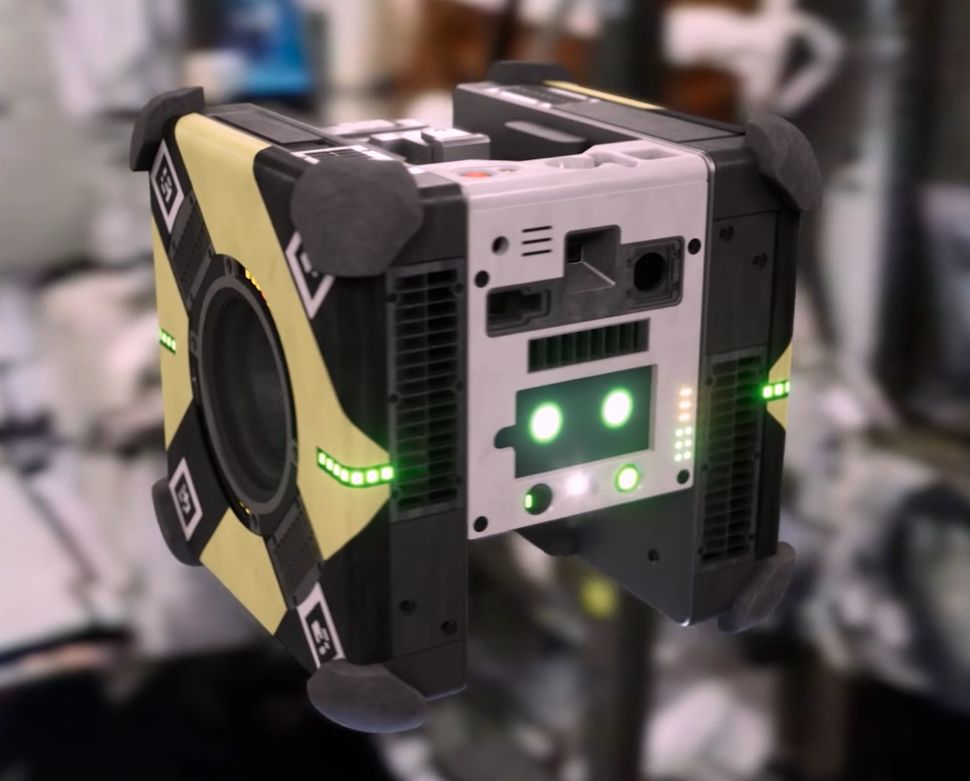
\includegraphics[width=0.75\linewidth]{Imagens/Astrobee NASA.png}
    \caption{Astrobee, robô auxiliar dos pesquisadores na ISS. Fonte: Space (\url{https://www.space.com/astrobee-robots-on-space-station.html}).}
    \label{fig:AstrobeeFoto}
\end{figure}

Este robô também serve como uma plataforma de teste para novas tecnologias espaciais, os pesquisadores podem carregar e testar software personalizado nos robôs para simular cenários de futuras missões espaciais. Essa plataforma de testes de sistemas está ajudando a NASA a desenvolver soluções para operações em estações espaciais futuras, incluindo a Gateway Lunar, que será utilizada em missões no espaço profundo \citep{nasaAstrobee}.

\subsection{Docking autônomo da Dragon 2}

A espaçonave Dragon 2, cujo desenvolvimento foi iniciado no primeiro semestre de 2013 pela SpaceX \citep{spaceDragonAlien}, é projetada para transportar tanto cargas quanto tripulações humanas ao espaço. Essa versão do modelo original, Dragon 1, apresenta melhorias em termos de autonomia, segurança e capacidade operacional. A Dragon 2 pode transportar até sete tripulantes ou uma combinação de cargas e tripulantes, permitindo seu uso em diferentes tipos de missões espaciais, como transporte para a ISS e outras operações em órbita baixa da Terra.

Entre as principais melhorias em relação à Dragon 1, está o sistema de lançamento e retorno. A Dragon 2 é equipada com motores SuperDraco, que oferecem capacidade de abortagem de emergência, aumentando a segurança durante o lançamento. Esse sistema permite que a espaçonave escape em caso de falhas no foguete, protegendo a tripulação. Além disso, a Dragon 2 utiliza paraquedas redesenhados para garantir um pouso mais controlado, uma atualização em relação ao modelo anterior, que dependia de procedimentos diferentes para retornar à Terra.

Outra inovação é o sistema de navegação autônoma \citep{nasaStarshipDocking}, que permite acoplamento direto à ISS sem a necessidade do braço robótico Canadarm2. Essa funcionalidade reduz a complexidade das operações e melhora a eficiência das missões. A Dragon 2 também apresenta um design interno atualizado, com controles interativos por touchscreen e maior adaptação para longas estadias, oferecendo mais conforto e funcionalidade para os tripulantes.

\begin{figure}[H]
    \centering
    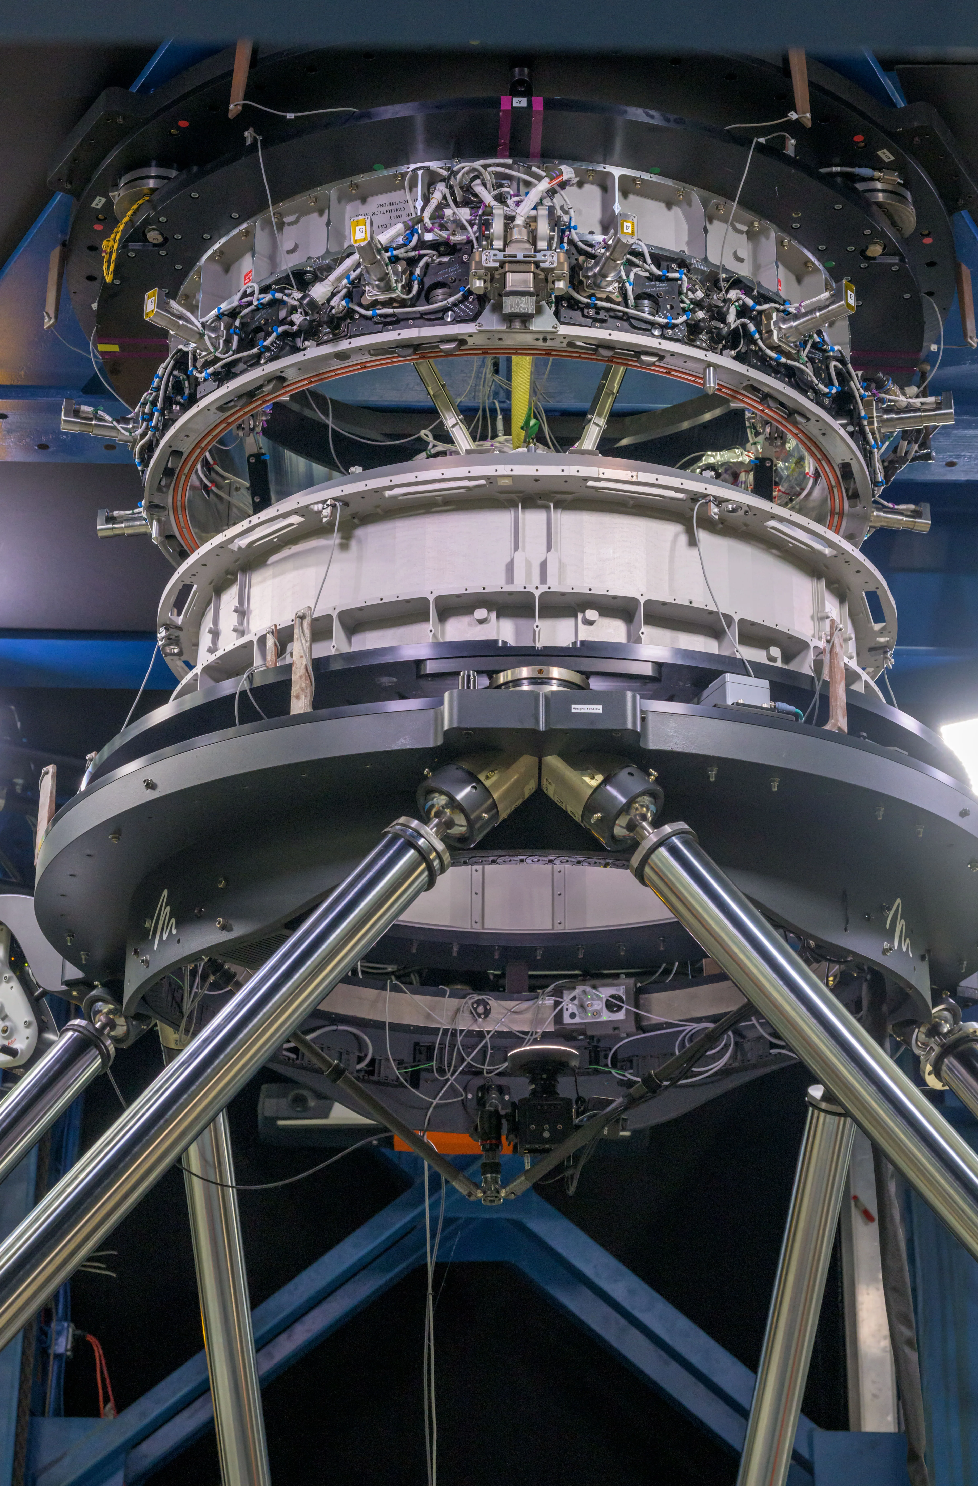
\includegraphics[width=0.75\linewidth]{Imagens/Docking system.png}
    \caption{Sistema de docking sendo testado pela NASA e SpaceX. Fonte: Nasa \url{https://www.nasa.gov/image-article/nasa-spacex-test-starship-lunar-lander-docking-system/}.}
    \label{fig:TesteDockingFoto}
\end{figure}

Além disso, a Dragon 2 é reutilizável, o que contribui para a redução dos custos operacionais em comparação com espaçonaves descartáveis. Essa característica está alinhada com a filosofia da SpaceX de tornar as viagens espaciais mais acessíveis e sustentáveis. No entanto, áreas como a ampliação de sua capacidade de carga e a adaptação para missões em espaço profundo ainda podem ser exploradas.

A Dragon 2 reflete avanços tecnológicos no transporte espacial comercial e é uma alternativa para missões que exigem flexibilidade operacional. Suas capacidades e inovações contribuem para o aumento das operações humanas em órbita terrestre e futuras explorações espaciais.

\subsection{Sustentabilidade e gerenciamento de detritos}

À medida que o número de objetos em órbita aumenta, a estabilidade do ambiente operacional se torna uma preocupação cada vez maior. Nos últimos anos, uma grande quantidade de detritos espaciais se acumulou com os satélites e naves espaciais lançados ao espaço, representando risco para futuras missões e para a integridade das operações deles. O lixo espacial varia de grandes pedaços de foguetes desativados a detritos de colisões e explosões em órbita. Estima-se que atualmente existam mais de 670.000 objetos maiores que 1 cm na órbita da Terra \citep{esaSpaceDebris}, com milhões de objetos menores representando sérios riscos. O problema é agravado pelo uso de satélites de órbita baixa, como os projetos Starlink e OneWeb, que prometem melhorar a conectividade global. Embora estas medições tenham revelado resultados importantes, também aumentaram o risco de colisão à medida que aumentaram a densidade dos objetos no espaço orbital crítico. Impactos de alta velocidade, conforme explica \citep{esaAboutSpaceDebris} podem criar milhares de fissuras, levando a um problema maior e a uma condição conhecida como síndrome de Kessler, onde colisões acontecem em cascata e se propagam sequencialmente, causando inutilização de certas órbitas por muitos anos ou até séculos \citep{kessler1978}.

Além dos riscos de acidentes, os locais de resíduos também têm impactos financeiros e operacionais. As empresas e agências espaciais precisam investir em manutenção e manutenção preventiva para proteger suas aeronaves. Esses processos aumentam os custos operacionais, causando consumo de combustível e encurtando a vida útil do satélite. Por outro lado, a falta de gerenciamento adequado de detritos pode danificar ativos e levar a interrupções econômicas na indústria orbital.

A gestão de resíduos requer cooperação internacional. Medidas como melhorar dispositivos eletrônicos de escuta, como redes e robôs de captura, e implementar padrões mais rigorosos para remoção de satélites são passos importantes para reduzir o problema. Organizações como a ESA e a NASA também estão promovendo projetos sustentáveis \citep{esaDebrisMitigation2023}, incentivando o uso de materiais que queimam completamente na reentrada e sistemas que garantem a segurança dos satélites no final de sua jornada.

\subsection{MEV}

O Mission Extension Vehicle-1 (MEV-1), desenvolvido pela Northrop Grumman, é uma espaçonave pioneira projetada para estender a vida útil de satélites em órbita geossíncrona. Lançado em 9 de outubro de 2019, o MEV-1 realizou sua primeira missão ao se acoplar ao satélite Intelsat 901 \citep{nytMEV1}, que havia excedido sua vida operacional. O MEV-1 utiliza um mecanismo de captura que se conecta ao motor principal do satélite cliente, assumindo o controle de suas operações de atitude e órbita. Essa tecnologia permite que satélites que de outra forma seriam desativados continuem em operação, reduzindo a necessidade de lançar novos satélites e contribuindo para a sustentabilidade das operações espaciais. Além de sua capacidade de extensão de vida útil, o MEV-1 demonstra avanços significativos em operações de proximidade e acoplamento em órbita, estabelecendo um novo padrão para serviços de manutenção espacial \citep{mev1}.

\subsection{Missões de exploração}

O programa Artemis, liderado pela NASA, busca estabelecer uma presença sustentável ao redor da Lua e na sua superfície \citep{nasaArtemis}, o que requer o desenvolvimento de tecnologias avançadas para operações de rendezvous and docking or berthing (RVD/B) em ambientes conectados. Ao contrário das operações em órbita baixa da Terra, as missões lunares apresentam desafios únicos pois a distância entre a Lua e a Terra pode causar atrasos nas comunicações de alguns segundos \citep{keeports2006}. Isso limita as oportunidades de controle humano imediato, exigindo sistemas autônomos robustos e confiáveis para executar tarefas críticas como o rendezvous and docking entre espaçonaves, módulos espaciais e outros.

Para superar essas limitações, os sistemas RVD/B na superfície lunar são usados com autonomia robótica aprimorada, permitindo que eles realizem procedimentos complexos de forma independente. Sensores avançados, como LiDAR \citep{farkasvolgyi2023} e câmeras estereoscópicas, combinados com algoritmos de aprendizado de máquina e processamento de dados em tempo real, permitem que as espaçonaves detectem objetos \citep{ibmComputerVision}, calculem caminhos de aproximação e façam ajustes durante a aproximação ou falha sem a necessidade de assistência imediata da gerência de solo. Essa autonomia é essencial não apenas para a segurança das operações, mas também para maximizar a eficiência em missões onde a janela de oportunidade para manobras é limitada \citep{fehse2003}.

A tecnologia desenvolvida para o programa Artemis tem aplicações diretas em futuras missões de exploração a Marte e outras partes do sistema solar que terão uma vida útil muito mais longa. A integração de sistemas autônomos de RVD/B representa um avanço significativo nas capacidades humanas de operar em ambientes espaciais desafiadores, promovendo a sustentabilidade das missões e reduzindo a dependência de intervenções diretas. Esses avanços também servem como base para o desenvolvimento de infraestrutura orbital lunar, como a estação Gateway, que desempenhará um papel central no suporte às missões do programa Artemis e além \citep{nasaGateway}.
